% =====================================================================
%  NLDB 2026 -- 15-minute talk
%  Towards Robust Uzbek Neural Dependency Parsing: Cross-Treebank Training
%  Author: Sanatbek Matlatipov (National University of Uzbekistan)
%  Built on the LDV beamer theme (see example.tex / ldvtheme/).
%
%  LOGOS: drop two files into THIS folder to brand the header:
%     nuu-logo.png   (left)   and   nldb-logo.png  (right)
%  Until then a plain text fallback is shown (the deck still compiles).
%
%  Compile:  latexmk -pdf presentation.tex      (or pdflatex x2)
% =====================================================================
\documentclass{beamer}
\mode<presentation>
{
  \usetheme{ldv}
  \setbeamercovered{transparent}
  \setbeamertemplate{navigation symbols}{} % clean look
}

\usepackage[utf8]{inputenc}
\usepackage[T1]{fontenc}
\usepackage{amsmath,amssymb,amsfonts}
\usepackage{times}
\usepackage{graphicx}
\usepackage{booktabs}
\usepackage{array}
\usepackage{colortbl}
\usepackage{tabularx}
\usepackage{tikz}
\usepackage{tikz-dependency}
\usepackage{pgfplots}
\pgfplotsset{compat=1.18}
\usetikzlibrary{arrows.meta, positioning, fit, calc,
                shapes.geometric}
\usepackage{hyperref}

% ---- Header / footer macros required by the ldv theme ----------------
\newcommand{\slidenomenclature}{Slide}
\newcommand{\zwischentitel}{Robust Uzbek Dependency Parsing}
\newcommand{\leitthema}{S.\,Matlatipov (NUU)}
\newcommand{\presdatum}{NLDB 2026 \, $\vert$ \, 18 June}

% ---- Replace the TUM logos in the headline with NUU / NLDB -----------
\setbeamertemplate{headline}{%
  \vspace{0.15cm}%
  \begin{tabularx}{\paperwidth}[t]{lXr}
    \hspace{0.25cm}%
    \IfFileExists{nuu-logo.png}%
      {
\includegraphics[height=0.85cm]{nuu-logo.png}}%
      {\raisebox{0.15cm}{\textcolor{beamer@blendedblue}{\small\textbf{NUU}}}}%
    & &
    \IfFileExists{nldb-logo.png}%
      {
\includegraphics[height=0.85cm]{nldb-logo.png}}%
      {\raisebox{0.15cm}{\textcolor{beamer@blendedblue}{\small\textbf{NLDB~2026}}}}%
    \hspace{0.25cm}%
  \end{tabularx}%
  \par\nointerlineskip
  \parbox{\paperwidth}{\vspace{0.7mm}\hspace{0.18cm}%
    \textcolor{beamer@blendedblue}{\rule{0.955\paperwidth}{0.4pt}}}%
}

% ---- Title metadata --------------------------------------------------
\title{Towards Robust Uzbek Neural Dependency Parsing}
\subtitle{Cross-Treebank Training \& Linguistically-Motivated Subword Fusion}
\author{Sanatbek Matlatipov}
\institute{National University of Uzbekistan named after Mirzo Ulugbek\\
  \texttt{s.matlatipov@nuu.uz}}
\date{NLDB 2026 \ $\vert$ \ 18 June 2026}

% A couple of convenience colours pulled from the theme palette
% (tumcolor-blue / -green / -orange / -lightgrey are defined by ldv).

\begin{document}

% =====================================================================
% 1. Title
% =====================================================================
\begin{frame}
  \titlepage
\end{frame}

% =====================================================================
% 2. Outline (sections only -- kept intentionally minimal)
% =====================================================================
\begin{frame}{Outline}
  \tableofcontents[subsectionstyle=hide]
\end{frame}

% =====================================================================
\section{Introduction}
% =====================================================================

% --- 3. Uzbek Language I (background) ---------------------------------
\begin{frame}{Uzbek Language I}
\begin{columns}[T]
\column{0.52\textwidth}
\footnotesize
\begin{itemize}\setlength\itemsep{4pt}
  \item \textbf{Growing NLP interest}, yet still under-resourced
        compared to major world languages.
  \item \textbf{Low-Resource}: NLP resources are sparse and low density.
  \item \textbf{Our language is Uzbek}:
        \begin{itemize}\setlength\itemsep{2pt}
          \item Official language of Uzbekistan.
          \item Native to Central Asia, Afghanistan, Russia, and Xinjiang (China).
          \item \textbf{Spoken by 40 million} people (as of 2026).
        \end{itemize}
\end{itemize}
\column{0.48\textwidth}
\centering
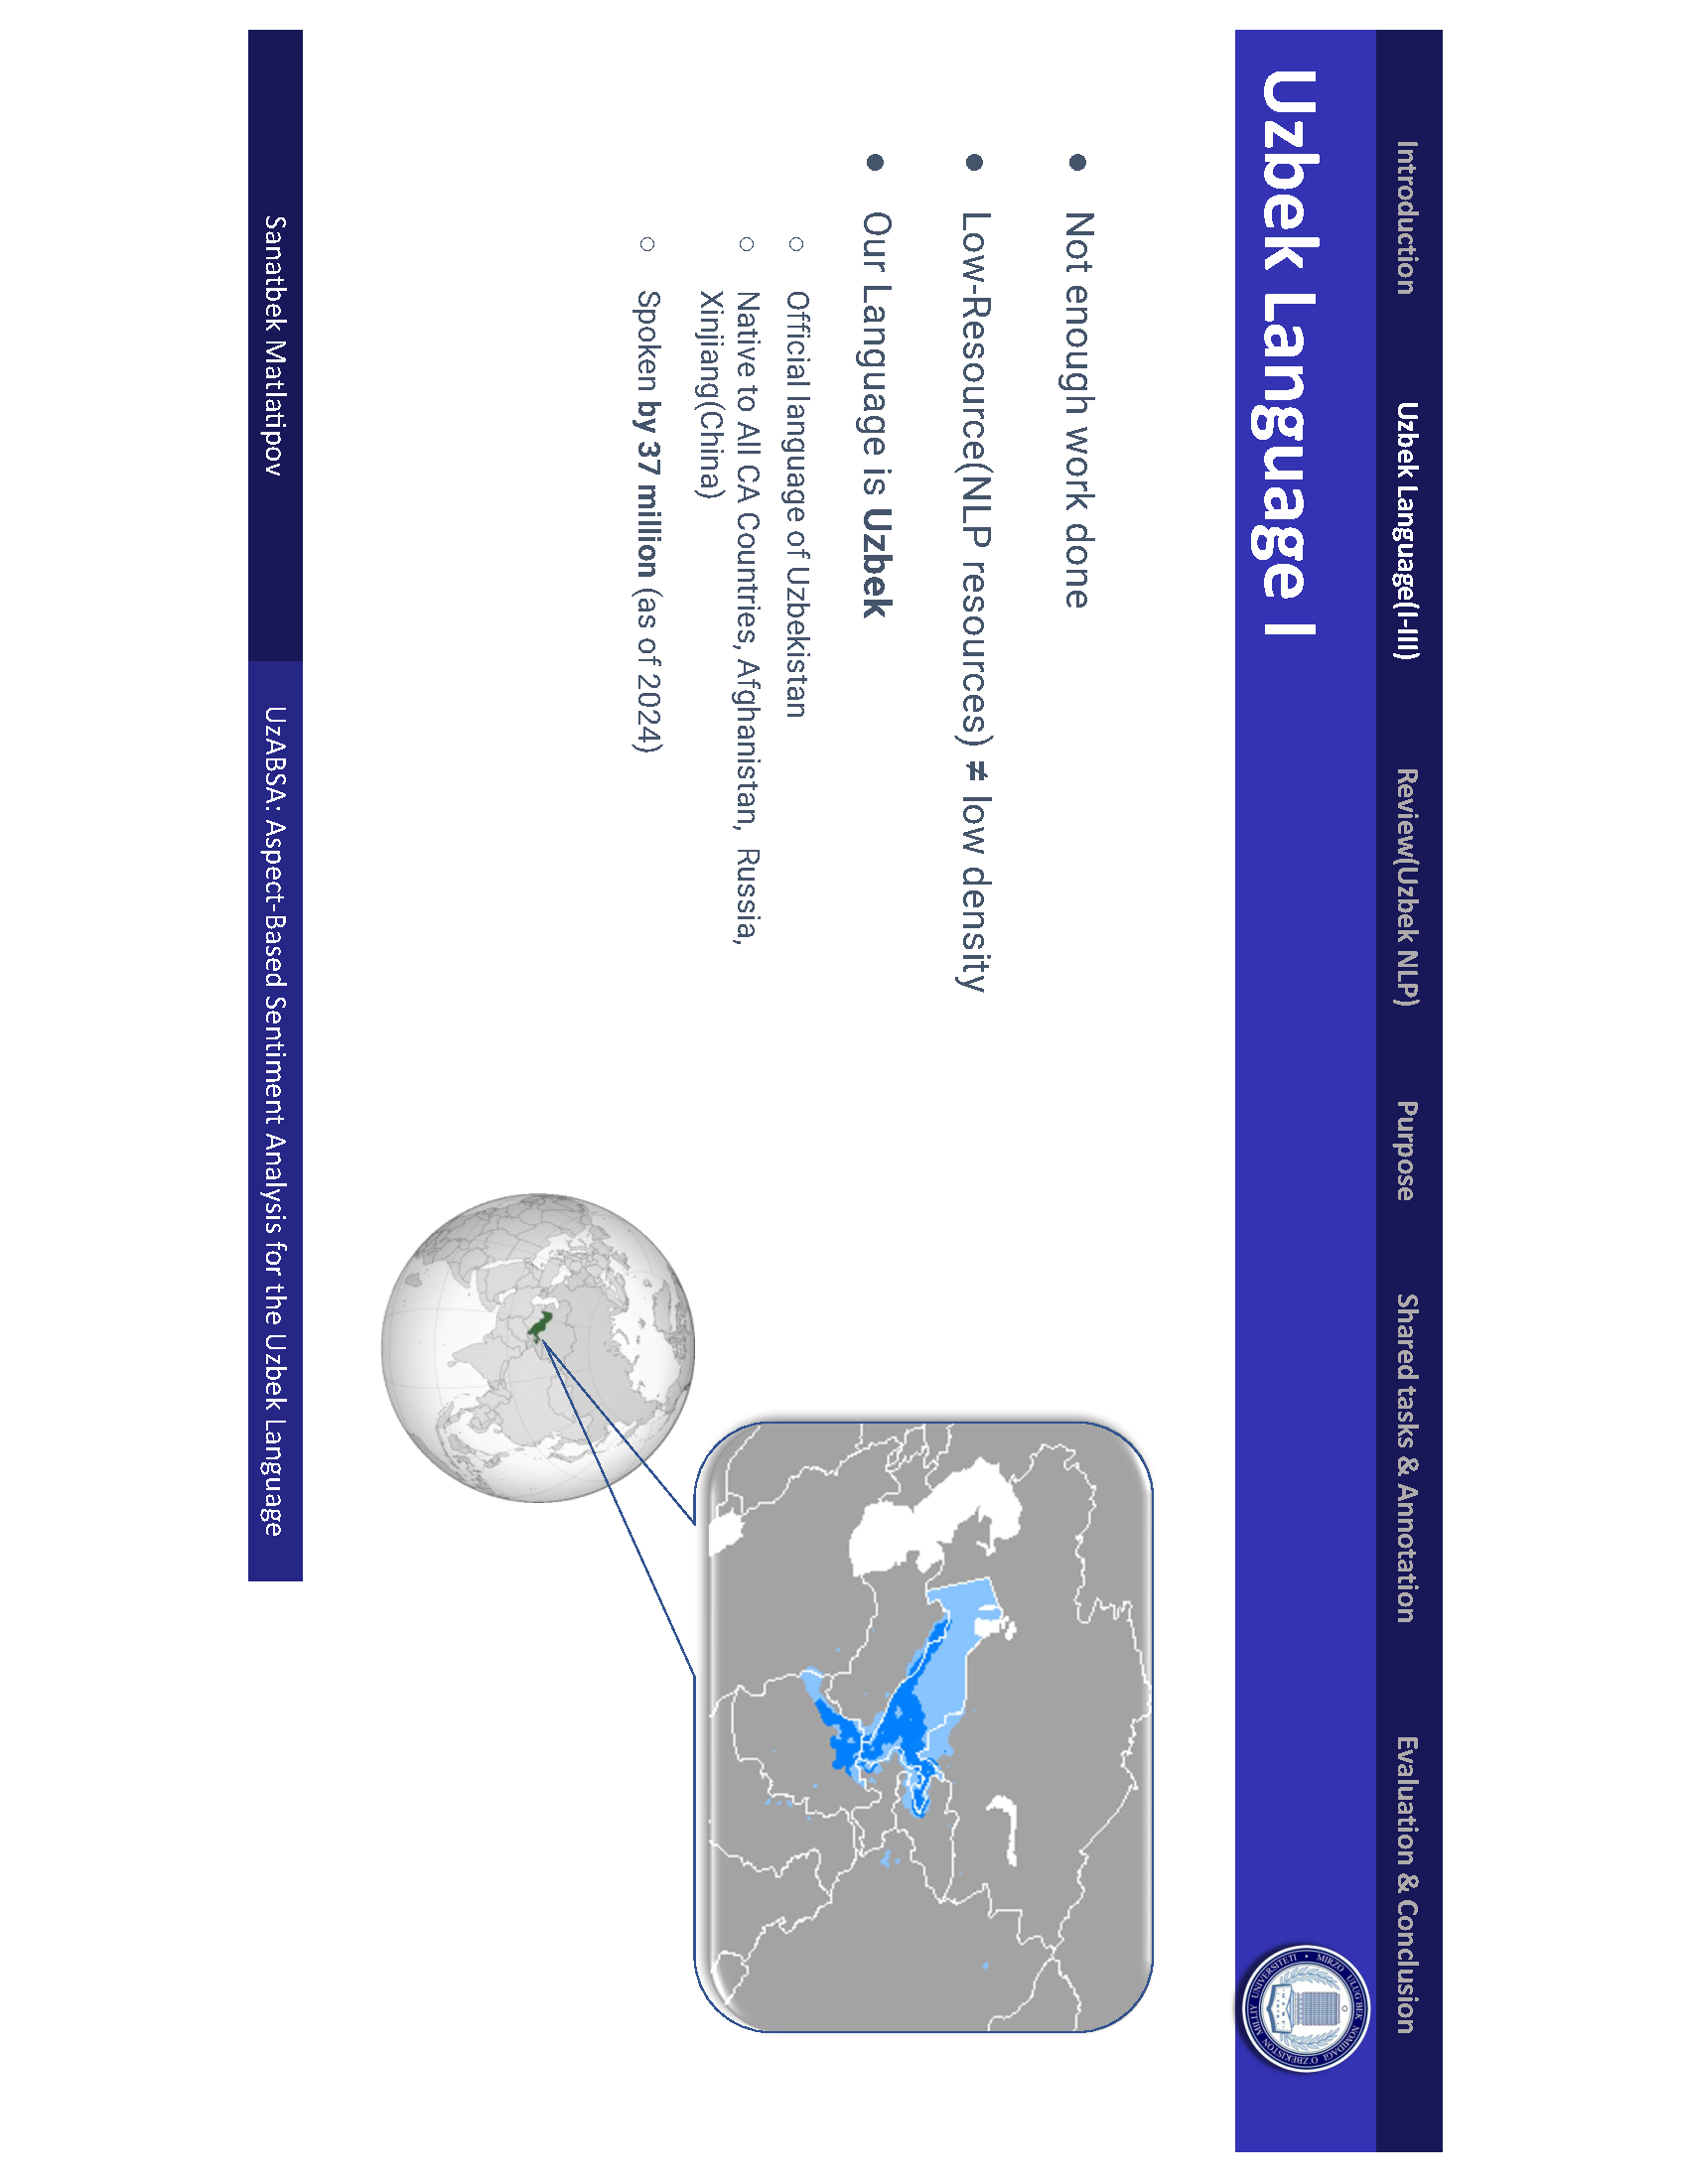
\includegraphics[width=0.95\textwidth]{uzbek_map.png}
\end{columns}
\end{frame}

% --- 4a. Motivation: the linguistic challenges -----------------------
\begin{frame}[t]{Why is Uzbek dependency parsing hard?}
\begin{columns}[T]
\column{0.6\textwidth}
\footnotesize
\begin{itemize}\setlength\itemsep{4pt}
  \item \textbf{Agglutinative}: long suffix chains encode case, tense,
        person, evidentiality.
  \item \textbf{Flexible word order} and strong genre variation.
  \item \textbf{Low-resource}: fewer than $1{,}000$ manually annotated
        UD sentences.
\end{itemize}
\column{0.4\textwidth}
\footnotesize
\begin{block}{Turkic features}
\begin{itemize}\setlength\itemsep{2pt}
  \item Null subject (pro-drop).
  \item No articles or grammatical gender.
  \item SOV word order.
\end{itemize}
\end{block}
\end{columns}
\vspace{0.1cm}
\begin{center}
\includegraphics[width=0.80\textwidth,height=0.33\textheight,keepaspectratio]%
  {uzbek_sample.jpg}
\end{center}
\vspace{-0.15cm}
{\centering\scriptsize
\textit{One Uzbek word $=$ a whole English sentence} --- agglutination,
plus scarce data, defines our two challenges.\par}
\note{
\textbf{Frame the problem (1 min)}
\begin{itemize}
  \item Agglutination is the core difficulty: a single word can pack
        root + plural + case, so the parser must handle long suffix
        chains rather than isolated words.
  \item Point at the figure: \textit{kelmaganlardanmisizlar?} --- one
        Uzbek word --- unpacks into eight English words, ``Are you one of
        those who didn't come?''  That density is what the parser faces.
  \item Flexible word order plus an SOV default means long-distance
        dependencies are common — the verb sits at the end, and with
        pro-drop the subject is often absent.
  \item Fewer than 1\,000 annotated UD sentences existed for the whole
        language before our work — this is the data bottleneck.
  \item Set up the two levers: better \emph{representations} for the
        morphology, more \emph{data} for the scarcity. Next slide shows
        \emph{why} morphology matters so much.
\end{itemize}
}
\end{frame}

% --- 4b. Hook: suffixes drive the syntax -----------------------------
\begin{frame}[t]{Suffixes carry the syntax}
\begin{columns}[T]
\column{0.46\textwidth}
\footnotesize
A single suffix can determine the dependency relation:
\vspace{0.3cm}
\begin{block}{Morphology breakdown}
\small
\textit{bolalar\textcolor{tumcolor-orange}{ning}} = ``of the children''\\[4pt]
bola $+$ lar\,(\textsc{pl}) $+$
\textcolor{tumcolor-orange}{\textbf{ning}\,(\textsc{gen})}
\end{block}
\vspace{0.2cm}
The \textcolor{tumcolor-orange}{\textbf{-ning}}\,(\textsc{gen}) suffix
alone drives the \texttt{nmod:poss} arc.
\column{0.54\textwidth}
\centering
\resizebox{\linewidth}{!}{%
\begin{dependency}[theme=simple,
                   edge style={black!85, line width=0.7pt},
                   label style={font=\small, fill=white, inner sep=1.5pt}]
  \begin{deptext}[column sep=0.55cm, row sep=0.12cm]
    bolalar\textcolor{tumcolor-orange}{\textbf{ning}} \& kitobi \& keldi \\
    NOUN \& NOUN \& VERB \\
  \end{deptext}
  \depedge{2}{1}{nmod:poss}
  \depedge{3}{2}{nsubj}
  \deproot{3}{root}
\end{dependency}}\\[6pt]
{\footnotesize \textit{``the children's book arrived''}}\\[4pt]
{\tiny Example of a manually annotated UzUDT dependency tree.}
\end{columns}
\note{
\textbf{The key intuition (1 min)}
\begin{itemize}
  \item This is the heart of the motivation: morphology \emph{directly}
        drives syntax. Strip the \textbf{-ning} genitive suffix and the
        possessive relation disappears.
  \item Walk the tree: \textit{bolalarning} (genitive) modifies
        \textit{kitobi} via \texttt{nmod:poss}; that noun phrase is the
        subject of \textit{keldi} (``arrived'').
  \item Take-away: a parser that ignores the rightmost suffix loses the
        syntactic signal. This motivates our \emph{last-subword fusion}
        later in the talk.
\end{itemize}
}
\end{frame}

% --- 5. The gap ------------------------------------------------------
\begin{frame}{The gap and our approach}
\textbf{Problem.} Existing Uzbek UD treebanks are small; neural parsers
need both \emph{more data} \emph{and} \emph{better representations}.
\vspace{0.35cm}
\begin{columns}[T]
\column{0.5\textwidth}
\begin{block}{New resource}
\textbf{UzUDT} --- 684 gold UD sentences (largest for Uzbek).
\end{block}
\column{0.5\textwidth}
\begin{block}{Two lightweight strategies}
\begin{enumerate}
  \item Last-subword \textbf{fusion} (suffix-aware).
  \item \textbf{Cross-treebank} training (merge genres).
\end{enumerate}
\end{block}
\end{columns}
\vspace{0.25cm}
\centering\footnotesize
No heavy architecture changes --- efficient and low-resource-friendly.
\end{frame}

% --- 6. Contributions + teaser ---------------------------------------
\begin{frame}{Contributions}
\begin{enumerate}\setlength\itemsep{4pt}
  \item \textbf{UzUDT}: a new 684-sentence gold Uzbek UD treebank
        (INCEpTION, 6 annotators, full adjudication).
  \item \textbf{Last-subword fusion}: a linguistically-motivated
        WordPiece$\to$UD-token alignment.
  \item \textbf{Cross-treebank training}: merging genre-complementary
        Uzbek treebanks.
  \item \textbf{Controlled factorial study}
        (3 configs $\times$ 2 data $=$ 6 runs) $+$ released code and
        12 checkpoints.
\end{enumerate}
\vspace{0.15cm}
\begin{block}{Headline result}
\centering
Best system \textbf{85.08 UPOS / 72.39 UAS / 63.81 LAS};
cross-treebank adds \textbf{$+9.62$ to $+11.16$ LAS}.
\end{block}
\end{frame}

% =====================================================================
\section{Related Work}
% =====================================================================
\begin{frame}{Related work}
\footnotesize
\begin{itemize}\setlength\itemsep{3pt}
  \item \textbf{Universal Dependencies}: cross-lingual syntactic
        annotation (de Marneffe et al., 2021).
  \item \textbf{Agglutinative parsing}: morphology-aware features help
        Turkish / Turkic (Eryi\u{g}it et al., 2008).
  \item \textbf{Uzbek UD}: UD\_Uzbek-UT ($\sim$500 sents); we add
        \textbf{UzUDT} (684).
  \item \textbf{Neural pipelines}: Stanza; biaffine parser
        (Dozat \& Manning, 2017); UDify (75 languages).
  \item \textbf{Uzbek encoders}: TahrirchiBERT (broad domain),
        BERTbek (news).
\end{itemize}
\vspace{0.3cm}
\begin{block}{Our niche}
\centering
Lightweight robustness for low-resource Uzbek:
\emph{suffix-aware fusion} $+$ \emph{cross-treebank data}.
\end{block}
\end{frame}

% =====================================================================
\section{Dataset}
% =====================================================================

% --- 7. UzUDT -------------------------------------------------------
\begin{frame}{UzUDT: a new gold Uzbek UD treebank}
\begin{columns}[T]
\column{0.54\textwidth}
\footnotesize
\begin{itemize}\setlength\itemsep{3pt}
  \item 684 sentences, $\sim$7.8k tokens.
  \item Genres: fiction $+$ academic.
  \item INCEpTION; 6 annotators (4 linguists $+$ 2 NLP engineers).
  \item Double annotation $+$ full adjudication.
  \item UPOS, XPOS, lemma, features, deprels (UD~v2).
\end{itemize}
\column{0.46\textwidth}
\centering\scriptsize\textbf{Inter-annotator agreement}\\[3pt]
\begin{tabular}{lcc}
\toprule
Layer & $\kappa$ & $\alpha$ \\
\midrule
Lemma    & 95.2 & 94.6 \\
UPOS     & 93.7 & 94.1 \\
Features & 90.8 & 89.9 \\
\bottomrule
\end{tabular}
\end{columns}
\vspace{0.3cm}
\centering\footnotesize
Currently the \textbf{largest publicly available Uzbek UD treebank}.
\end{frame}

% --- 8. UT + data settings ------------------------------------------
\begin{frame}{Second treebank \& data settings}
\footnotesize
\textbf{UD\_Uzbek-UT} (Akhundjanova \& Talamo, 2025): 500 sentences,
news $+$ fiction, semi-automatic with manual correction.
\vspace{0.35cm}
\centering
\begin{tabular}{llrrrr}
\toprule
Setting & Source & Train & Dev & Test & Total \\
\midrule
\texttt{.1} UzUDT only & UzUDT      & 451 & 45 & 188 & 684 \\
\texttt{.2} Merged     & UzUDT$+$UT & 781 & 78 & 325 & 1{,}184 \\
\bottomrule
\end{tabular}
\vspace{0.35cm}
\flushleft
Merging nearly \textbf{doubles} the training data
($451 \rightarrow 781$ sentences) --- a direct test of whether data
quantity is the bottleneck.
\end{frame}

% --- 9. Why complementary -------------------------------------------
\begin{frame}{Why the treebanks are complementary}
\begin{columns}[T]
\column{0.56\textwidth}
\centering
\begin{tikzpicture}
\begin{axis}[
  ybar, width=6.4cm, height=4.7cm, bar width=7pt,
  ymin=0, enlarge x limits=0.16,
  symbolic x coords={PROPN,PRON,advcl,comp:lvc},
  xtick=data,
  x tick label style={font=\tiny,rotate=20,anchor=east},
  tick label style={font=\tiny},
  ylabel={\tiny \% of tokens / relations},
  legend style={font=\tiny, at={(0.5,1.02)}, anchor=south,
                legend columns=2},
]
\addplot[fill=tumcolor-blue!55]
  coordinates {(PROPN,0.3)(PRON,6.0)(advcl,5.9)(comp:lvc,0.3)};
\addplot[fill=tumcolor-orange!65]
  coordinates {(PROPN,5.2)(PRON,3.3)(advcl,1.8)(comp:lvc,3.6)};
\legend{UzUDT, UT}
\end{axis}
\end{tikzpicture}
\column{0.44\textwidth}
\footnotesize
\begin{itemize}\setlength\itemsep{5pt}
  \item UT: many \textbf{PROPN} (news; $5.2\%$ vs $0.3\%$).
  \item UzUDT: more \textbf{PRON}; $4\times$ more \textbf{advcl}.
  \item UT: $10\times$ more \textbf{compound:lvc}.
\end{itemize}
\vspace{0.25cm}
$\Rightarrow$ genre-complementary, so merging fills each other's
syntactic gaps.
\end{columns}
\end{frame}

% =====================================================================
\section{Methodology}
% =====================================================================

% --- 10. Pipeline overview -------------------------------------------
\begin{frame}[fragile]{Pipeline: from text to a labeled tree}
\centering
\resizebox{\textwidth}{!}{%
\begin{tikzpicture}[
   node distance=6mm,
   stage/.style={rectangle, rounded corners, draw=black, thick,
                 align=center, minimum height=1.25cm, minimum width=2.1cm,
                 font=\small},
   io/.style={rectangle, draw=black!55, fill=black!5, align=center,
              minimum height=1.05cm, font=\small},
   arr/.style={-{Stealth[length=3mm]}, thick}
  ]
  \node[io] (in) {UD-tokenized\\Uzbek sentence};
  \node[stage, fill=tumcolor-blue!20,   right=of in]  (enc)
        {Encoder\\{\scriptsize FastText /}\\{\scriptsize TahrirchiBERT}};
  \node[stage, fill=tumcolor-orange!28, right=of enc] (fus)
        {Subword$\to$Token\\Fusion};
  \node[stage, fill=tumcolor-green!28,  right=of fus] (tag)
        {Joint Tagger\\{\scriptsize UPOS/XPOS/UFeats}};
  \node[stage, fill=tumcolor-blue!32,   right=of tag] (par)
        {Biaffine\\Parser};
  \node[io, right=of par] (out) {Labeled\\UD tree};
  \draw[arr] (in)--(enc);
  \draw[arr] (enc)--(fus);
  \draw[arr] (fus)--(tag);
  \draw[arr] (tag)--(par);
  \draw[arr] (par)--(out);
  \draw[arr, dashed, tumcolor-green!60!black]
        (tag.south) .. controls +(0,-1.0) and +(0,-1.0) .. (par.south);
  \node[font=\scriptsize, tumcolor-green!55!black]
        at ($(tag.south)!0.5!(par.south)+(0,-0.78)$) {predicted UPOS};
\end{tikzpicture}}

\vspace{0.45cm}
\footnotesize
Encoder is \textbf{frozen}; fusion maps WordPieces to UD tokens;
training is \textbf{sequential} (tagger first, then parser on
\emph{re-tagged} data --- no gold-tag leakage).
\end{frame}

% --- 11. Token representation ---------------------------------------
\begin{frame}{Token representation: four channels}
Each UD token is represented by a concatenation of four vectors:
\begin{equation*}
  \mathbf{x}_i = \big[\,
    \underbrace{\mathbf{e}_{\text{word}}(w_i)}_{\text{static}};\;
    \underbrace{\mathbf{e}_{\text{char}}(w_i)}_{\text{char-LSTM}};\;
    \underbrace{\mathbf{e}_{\text{upos}}(\hat p_i)}_{\text{predicted}};\;
    \underbrace{\mathbf{e}_{\text{ctx}}(w_i)}_{\text{fused BERT}}
  \,\big]
\end{equation*}
\centering
\begin{tikzpicture}[box/.style={minimum height=0.95cm, text width=2.2cm,
  align=center, draw=black, font=\scriptsize}, node distance=2mm]
  \node[box, fill=tumcolor-blue!20]       (w) {word\\\textbf{300}\,d};
  \node[box, fill=tumcolor-lightgrey!70, right=of w] (c) {char\\LSTM};
  \node[box, fill=tumcolor-green!28, right=of c]     (p) {UPOS\\\textbf{50}\,d};
  \node[box, fill=tumcolor-orange!28, right=of p]    (x) {ctx (BERT)\\\textbf{768}\,d};
\end{tikzpicture}

\vspace{0.25cm}
\footnotesize
\begin{itemize}\setlength\itemsep{2pt}
  \item \textbf{FastText config:} word channel is static 300-d; \emph{no}
        ctx channel.
  \item \textbf{TahrirchiBERT config:} ctx channel is a 768-d fused
        vector (next slide).
\end{itemize}
\end{frame}

% --- 12. KEY: subword-to-token fusion -------------------------------
\begin{frame}{Subword$\to$token fusion: our key heuristic}
\footnotesize\textbf{Problem:} BERT WordPieces $\neq$ UD tokens --- we
must aggregate $\{h_1,\dots,h_k\}$ into one vector per token.
\vspace{0.1cm}
\centering
\begin{tikzpicture}[
  tok/.style={rectangle, rounded corners, draw, thick,
              minimum width=2.4cm, minimum height=0.7cm, font=\small},
  sw/.style={rectangle, draw, minimum width=1.4cm, minimum height=0.7cm,
             font=\small},
  arr/.style={-{Stealth[length=2.5mm]}, thick}
 ]
  \node[tok, fill=tumcolor-lightgrey!60] (word) {\textit{bolalarning}};
  \node[sw] (s1) [below=1.1cm of word, xshift=-1.9cm] {bola};
  \node[sw, right=0.25cm of s1] (s2) {\#\#lar};
  \node[sw, fill=tumcolor-orange!40, right=0.25cm of s2] (s3) {\#\#ning};
  \node[font=\scriptsize, below=0.4mm of s1] {$h_1$};
  \node[font=\scriptsize, below=0.4mm of s2] {$h_2$};
  \node[font=\scriptsize, below=0.4mm of s3] {$h_3$};
  \draw[arr] (word.south) -- (s1.north);
  \draw[arr] (word.south) -- (s2.north);
  \draw[arr] (word.south) -- (s3.north);
  \node[tok, fill=tumcolor-green!28, right=2.0cm of s3]
        (ectx) {$\mathbf{e}_{\text{ctx}}(t)$};
  \draw[arr, tumcolor-orange!80!black] (s3.east) -- (ectx.west);
  \node[font=\scriptsize] at ($(s3.east)!0.5!(ectx.west)+(0,0.28)$)
        {pick last};
\end{tikzpicture}

\vspace{0.15cm}
\begin{columns}[T]
\column{0.5\textwidth}
\centering\footnotesize\textbf{Last-subword (ours)}
\[ \mathbf{e}_{\text{ctx}}(t)=h_k \]
\scriptsize Rightmost piece $=$ outermost suffix
(\#\#ning $=$ \textsc{Gen}; \#\#siz $=$ 2\textsc{pl}).
\column{0.5\textwidth}
\centering\footnotesize\textbf{Mean pooling (baseline)}
\[ \mathbf{e}_{\text{ctx}}(t)=\tfrac{1}{k}\textstyle\sum_{i=1}^{k} h_i \]
\scriptsize Language-agnostic; dilutes the suffix signal.
\end{columns}
\end{frame}

% --- 13. Joint tagger -----------------------------------------------
\begin{frame}{Joint morphosyntactic tagger}
\centering
\begin{tikzpicture}[
  inp/.style={draw, minimum width=0.9cm, minimum height=0.6cm,
            fill=tumcolor-lightgrey!60, font=\scriptsize},
  lstm/.style={draw, minimum width=0.9cm, minimum height=0.6cm,
               fill=tumcolor-blue!22, font=\scriptsize},
  head/.style={draw, rounded corners, minimum width=1.5cm,
               minimum height=0.6cm, font=\scriptsize},
  arr/.style={-{Stealth[length=2mm]}, thick}
 ]
 \foreach \i in {1,2,3,4} {\node[inp]  (x\i) at (\i*1.4,0) {$x_{\i}$};}
 \foreach \i in {1,2,3,4} {\node[lstm] (l\i) at (\i*1.4,1) {};}
 \foreach \i in {1,2,3,4} {\draw[arr] (x\i)--(l\i);}
 \foreach \i/\j in {1/2,2/3,3/4} {\draw[<->, thick] (l\i)--(l\j);}
 \node[left=2mm of l1, font=\scriptsize] {BiLSTM};
 % Heads ordered [XPOS] [UFeats] [UPOS] so the exported UPOS sits on the
 % far right, next to the dashed box -> arrow never crosses the other heads.
 \node[head, fill=tumcolor-green!18] (xpos)  at (2.8,2.4) {XPOS};
 \node[head, fill=tumcolor-green!18] (feats) at (4.2,2.4) {UFeats};
 \node[head, fill=tumcolor-green!32] (upos)  at (5.7,2.4) {UPOS};
 \draw[arr] (l3.north) -- (xpos.south);
 \draw[arr] (l3.north) -- (feats.south);
 \draw[arr] (l3.north) -- (upos.south);
 \node[draw, dashed, text=tumcolor-green!50!black, right=1.0cm of upos,
       text width=2.0cm, align=center, font=\scriptsize] (exp)
       {predicted UPOS\\ $\to$ parser};
 \draw[arr, dashed, tumcolor-green!55!black] (upos.east) -- (exp.west);
\end{tikzpicture}

\vspace{0.35cm}
\footnotesize
A shared \textbf{BiLSTM} feeds three softmax heads. Only the
\textbf{predicted} UPOS embedding is exported to the parser.
\end{frame}

% --- 14. Biaffine parser --------------------------------------------
\begin{frame}{Deep biaffine dependency parser}
\begin{columns}[T]
\column{0.52\textwidth}
\centering
\begin{tikzpicture}[
  node distance=5mm,
  b/.style={draw, rounded corners, minimum width=2.4cm,
            minimum height=0.7cm, font=\scriptsize, align=center},
  arr/.style={-{Stealth[length=2mm]}, thick}
 ]
 \node[b, fill=tumcolor-lightgrey!60] (in)
      {BiLSTM states $r_i$\\{\tiny $+$ predicted UPOS emb.}};
 \node[b, fill=tumcolor-blue!22, below left=9mm and -2mm of in]  (mh)
      {MLP$^{\text{head}}$};
 \node[b, fill=tumcolor-blue!22, below right=9mm and -2mm of in] (md)
      {MLP$^{\text{dep}}$};
 \node[b, fill=tumcolor-orange!28, below=20mm of in] (bi)
      {Biaffine scorer};
 \node[b, fill=tumcolor-green!28, below=8mm of bi]   (out)
      {arc scores $+$ labels};
 \draw[arr] (in)--(mh); \draw[arr] (in)--(md);
 \draw[arr] (mh)--(bi); \draw[arr] (md)--(bi);
 \draw[arr] (bi)--(out);
\end{tikzpicture}
\column{0.48\textwidth}
\footnotesize\textbf{Dozat \& Manning (2017).}
\begin{itemize}\setlength\itemsep{2pt}
  \item BiLSTM states $\to$ head/dep subspaces via MLPs.
  \item Biaffine attention scores every head--dependent pair.
  \item Output: a labeled tree over UD tokens.
\end{itemize}
\vspace{0.15cm}
\centering
\resizebox{\linewidth}{!}{%
\begin{dependency}[theme=simple]
  \begin{deptext}[column sep=0.3cm]
    asarlar \& bizga \& eshigini \& ochib \& beradi \\
  \end{deptext}
  \depedge{5}{1}{nsubj}
  \depedge{5}{2}{obl}
  \depedge{5}{4}{xcomp}
  \depedge{4}{3}{obj}
  \deproot{5}{root}
\end{dependency}}
\end{columns}
\end{frame}

% =====================================================================
\section{Results \& Discussion}
% =====================================================================

% --- 15. Experiment matrix ------------------------------------------
\begin{frame}{Experiment matrix: 3 configs $\times$ 2 data settings}
\centering\small
\begin{tabular}{llllr}
\toprule
\textbf{Run} & \textbf{Embeddings} & \textbf{Fusion} & \textbf{Data}
  & \textbf{Train} \\
\midrule
E1.1 & FastText      & ---          & UzUDT      & 451 \\
E1.2 & FastText      & ---          & UzUDT$+$UT & 781 \\
E2.1 & TahrirchiBERT & Last-subword & UzUDT      & 451 \\
\rowcolor{tumcolor-green!22}
E2.2 & TahrirchiBERT & Last-subword & UzUDT$+$UT & 781 \\
E3.1 & TahrirchiBERT & Mean pooling & UzUDT      & 451 \\
E3.2 & TahrirchiBERT & Mean pooling & UzUDT$+$UT & 781 \\
\bottomrule
\end{tabular}

\vspace{0.3cm}
\footnotesize
\begin{itemize}\setlength\itemsep{2pt}
  \item \textbf{E1 vs E2}: embedding effect (static vs contextual).
  \item \textbf{E2 vs E3}: fusion effect (last-subword vs mean).
  \item \textbf{.1 vs .2}: data effect (cross-treebank augmentation).
\end{itemize}
\end{frame}

% --- 16. Main results tables ----------------------------------------
\begin{frame}{Main results (test set)}
\scriptsize
\begin{columns}[T]
\column{0.53\textwidth}
\centering\textbf{Tagging (accuracy \%)}\\[2pt]
\begin{tabular}{lrrr}
\toprule
Run & UPOS & XPOS & UFeats \\
\midrule
E1.1 & 79.19 & 79.81 & 66.61 \\
E1.2 & 80.26 & 83.20 & 66.98 \\
E2.1 & 82.45 & 80.90 & 65.37 \\
\rowcolor{tumcolor-green!22}
E2.2 & \textbf{85.08} & 84.72 & \textbf{71.09} \\
E3.1 & 82.76 & 81.37 & 65.22 \\
E3.2 & 84.02 & \textbf{87.07} & 70.39 \\
\bottomrule
\end{tabular}
\column{0.47\textwidth}
\centering\textbf{Parsing (accuracy \%)}\\[2pt]
\begin{tabular}{lrr}
\toprule
Run & UAS & LAS \\
\midrule
E1.1 & 69.57 & 51.24 \\
E1.2 & 72.27 & 62.40 \\
E2.1 & 72.05 & 54.19 \\
\rowcolor{tumcolor-green!22}
E2.2 & \textbf{72.39} & \textbf{63.81} \\
E3.1 & 69.10 & 51.55 \\
E3.2 & 70.74 & 60.05 \\
\bottomrule
\end{tabular}
\end{columns}
\vspace{0.25cm}
\centering\footnotesize
\textbf{E2.2} (BERT $+$ last-subword $+$ merged) wins 4 of 5 metrics;
only XPOS is best under mean pooling (E3.2).
\end{frame}

% --- 17. Three findings ---------------------------------------------
\begin{frame}{Three findings}
\begin{columns}[T]
\column{0.5\textwidth}
\centering
\begin{tikzpicture}
\begin{axis}[
  ybar, width=6.1cm, height=4.7cm, bar width=9pt,
  ymin=45, ymax=70, ylabel={LAS}, ylabel near ticks,
  symbolic x coords={E1.1,E1.2,E2.1,E2.2,E3.1,E3.2},
  xtick=data,
  x tick label style={rotate=45,anchor=east,font=\tiny},
  ytick={50,55,60,65}, tick label style={font=\tiny},
  nodes near coords,
  every node near coord/.append style={font=\tiny,rotate=90,anchor=west},
  enlarge x limits=0.12
]
\addplot[fill=tumcolor-blue!45]
  coordinates {(E1.1,51.24)(E1.2,62.40)(E2.1,54.19)
               (E2.2,63.81)(E3.1,51.55)(E3.2,60.05)};
\end{axis}
\end{tikzpicture}
\column{0.5\textwidth}
\footnotesize
\textbf{1. Contextual $>$ static.}\\
BERT vs FastText: UPOS $+4.82$ on merged data.\\[5pt]
\textbf{2. Fusion matters for parsing.}\\
Last-subword vs mean: LAS $+3.76$.\\
\scriptsize mean-BERT $60.05 <$ FastText $62.40 <$
\textbf{last-sub BERT $63.81$}.\\[5pt]
\normalsize\textbf{3. Cross-treebank is the biggest lever.}\\
\footnotesize LAS $+9.62$ (BERT), $+11.16$ (FastText).
\end{columns}
\end{frame}

% --- 18. Error analysis ---------------------------------------------
\begin{frame}{Error analysis (100 test sentences, E2.2)}
\begin{columns}[T]
\column{0.5\textwidth}
\scriptsize
\begin{tabular}{lr}
\toprule
Error type & \% \\
\midrule
PP/oblique attach.\     & 28 \\
Coordination scope      & 22 \\
Subordinate clauses     & 18 \\
Compound constructions  & 14 \\
Long-distance deps      & 10 \\
Other                   &  8 \\
\bottomrule
\end{tabular}
\vspace{0.2cm}\\
Top sources: \texttt{obl}/\texttt{nmod} ambiguity and coordination scope.
\column{0.5\textwidth}
\centering\scriptsize Missed light-verb construction:\\[4pt]
\resizebox{\linewidth}{!}{%
\begin{dependency}[theme=simple]
  \begin{deptext}[column sep=0.35cm]
    bolalar \& o'yinni \& davom \& etdi \& . \\
  \end{deptext}
  \depedge{4}{1}{nsubj}
  \depedge{4}{2}{obj}
  \depedge[edge style={blue}]{4}{3}{compound:lvc}
  \deproot{4}{root}
  \depedge[edge below, edge style={red,dashed}]{3}{1}{nsubj*}
  \depedge[edge below, edge style={red,dashed}]{4}{3}{obj*}
\end{dependency}}\\[4pt]
\scriptsize
\textcolor{blue}{Blue} $=$ gold \texttt{compound:lvc};
\textcolor{red}{red dashed} $=$ predicted error.
\end{columns}
\end{frame}

% =====================================================================
\section{Conclusion}
% =====================================================================

% --- 18. Conclusion -------------------------------------------------
\begin{frame}{Conclusion}
\begin{itemize}\setlength\itemsep{4pt}
  \item \textbf{UzUDT}: largest gold Uzbek UD treebank (684 sentences).
  \item \textbf{Cross-treebank} training is the dominant factor
        (LAS $+9.62$ to $+11.16$).
  \item \textbf{Last-subword fusion} is critical for parsing
        (LAS $+3.76$ over mean pooling).
  \item Best: TahrirchiBERT $+$ last-subword $+$ merged $=$
        \textbf{85.08 / 72.39 / 63.81} (UPOS / UAS / LAS).
\end{itemize}
\vspace{0.15cm}
\footnotesize
\textbf{Limitations:} small dev sets (45 / 78); UT genre mismatch and
validation noise.\\
\textbf{Future:} BERTbek, BERT$+$FastText fusion (E4--E7).\\[5pt]
Data \& 12 checkpoints:
\url{https://huggingface.co/Sanatbek/uzudt}\\
Code:
\url{https://github.com/SanatbekMatlatipov/robust-parsing-uzbek}
\end{frame}

% --- 19. Thank you --------------------------------------------------
\begin{frame}{}
\centering
\vspace{0.9cm}
{\Large \textcolor{beamer@blendedblue}{\textbf{Thank you!}}}\\[8pt]
Questions?\\[12pt]
\footnotesize
Sanatbek Matlatipov ---\ \texttt{s.matlatipov@nuu.uz}\\[2pt]
National University of Uzbekistan named after Mirzo Ulugbek
\end{frame}

% =====================================================================
\appendix
% =====================================================================
\begin{frame}{Appendix: parser training dynamics}
\centering
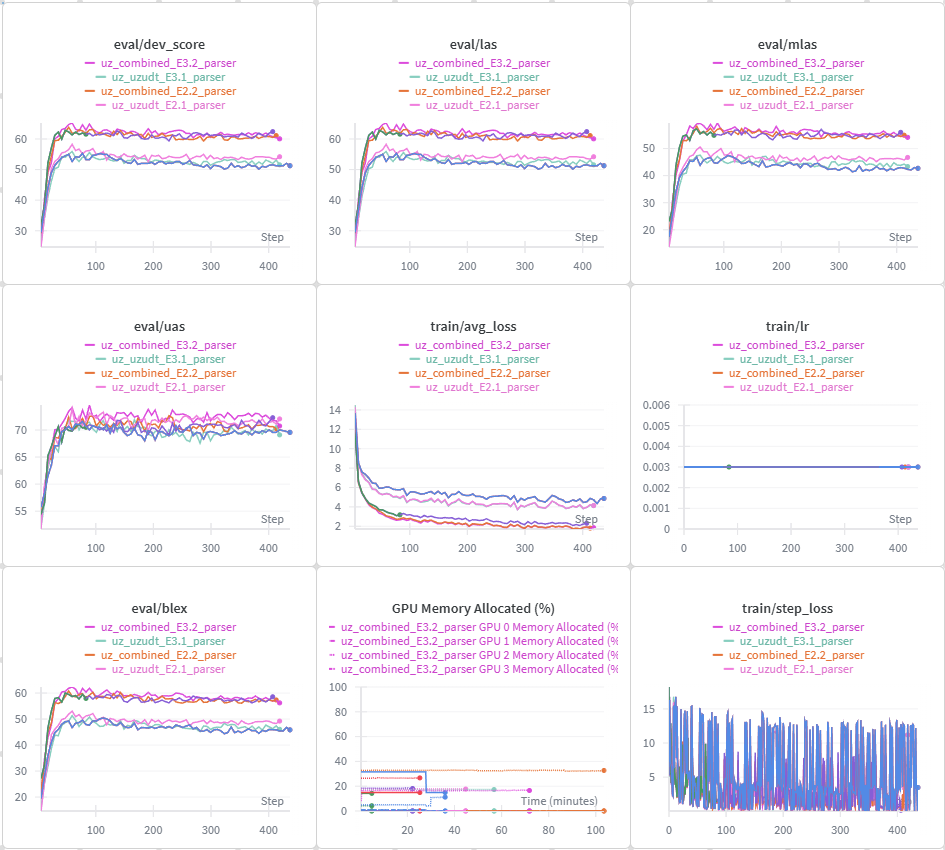
\includegraphics[width=0.92\textwidth,height=0.78\textheight,keepaspectratio]{uzbek-depparse.png}\\[2pt]
{\tiny Dev score and LAS/UAS/MLAS/BLEX over training steps
(UzUDT-only vs.\ merged).}
\end{frame}

\begin{frame}{Appendix: tagger training dynamics}
\centering
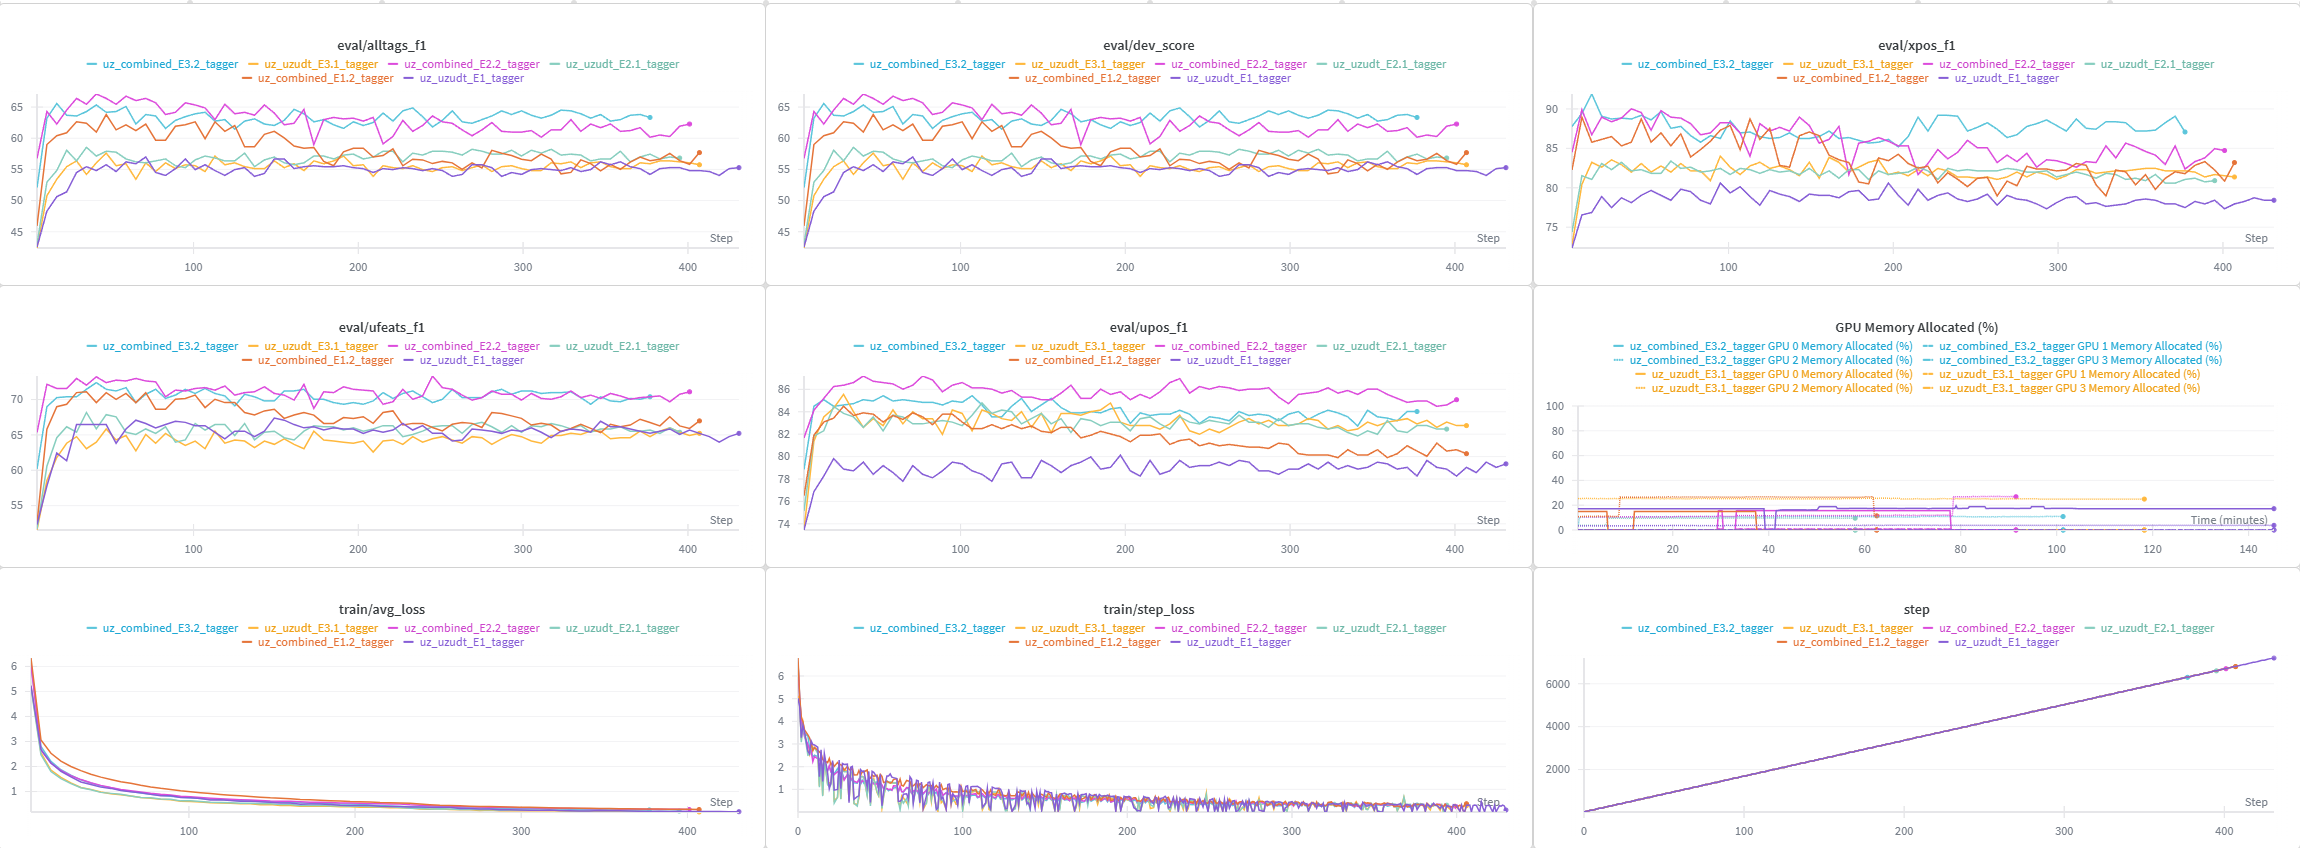
\includegraphics[width=0.96\textwidth,height=0.78\textheight,keepaspectratio]{uzbek-pos-tagger.png}\\[2pt]
{\tiny UPOS/XPOS/UFeats/AllTags F1 across the six runs.}
\end{frame}

\begin{frame}{Appendix: a correctly parsed sentence}
\centering
\resizebox{\textwidth}{!}{%
\begin{dependency}[theme=simple]
  \begin{deptext}[column sep=0.45cm]
    bu \& bo'limdagi \& asarlar \& bizga \& bu \& xazinaning \&
    eshigini \& ochib \& beradi \& . \\
    PRON \& ADJ \& NOUN \& PRON \& PRON \& NOUN \& NOUN \& VERB \&
    VERB \& PUNCT \\
  \end{deptext}
  \depedge{2}{1}{det}
  \depedge{3}{2}{amod}
  \depedge{9}{3}{nsubj}
  \depedge{9}{4}{obl}
  \depedge{6}{5}{det}
  \depedge{7}{6}{nmod:poss}
  \depedge{8}{7}{obj}
  \depedge{9}{8}{xcomp}
  \deproot{9}{root}
  \depedge{9}{10}{punct}
\end{dependency}}
\end{frame}

\end{document}
